\section{Datenanalyse}
\begin{frame}
\frametitle{Deskriptive Statistik}
Statistik wird üblicherweise in drei (nicht disjunkte) Bereiche eingeteilt:\\[0.2cm]
1. Deskriptive (beschreibende) Statistik:
\begin{itemize}[<+->]
\item Zusammenführung und Aufbereitung der Daten in Tabellen (sofern sinnvoll)
\item Visuelle Aufbereitung der Verteilung(en) der Daten durch Diagramme
\item Beschreibung der Daten durch Kennzahlen, wie Lagemaße, Streuungsmaße und Zusammenhangsmaße
\item Ziel: Beschreibung der Verteilungen von Merkmalen
\item Es sollen immer adäquate Methoden/Darstellungen verwendet werden und nicht-betrachtete Zusammenhänge/Informationen stets aufgeführt werden (Bsp.: Bei einem Streudiagramm werden mehrfache gleiche Punkte nicht dargestellt)
\end{itemize}
\end{frame}
\begin{frame}
\frametitle{Induktive Statistik}
2. Induktive (schließende) Statistik:
\begin{itemize}[<+->]
\item Induktion allgemein: Schließen vom Speziellen aufs Allgemeine
\item Ableiten von Eigenschaften der Grundgesamtheit aus einer Stichprobe
\item Grundlage bildet die Wahrscheinlichkeitstheorie
\item Eins der Hauptgebiete ist die Schätztheorie, z.B. Schätzen von Parametern (etwa Maximum-Likelihood-Schätzer) oder Schätzen von Konfidenzintervallen
\item Durchführung von Hypothesentests (Überprüfen einer Hypothese anhand von Beobachtungen)
\end{itemize}
\end{frame}
\begin{frame}
\frametitle{Explorative Statistik}
3. Explorative (erkundende) Statistik:
\begin{itemize}[<+->]
\item Aufdecken möglicher Zusammenhänge innerhalb von gegebenen Daten
\item Meist sind in den zugrunde liegenden Daten wenige Zusammenhänge bekannt
\item Formulierung und statistische Analyse/Bewertung von Hypothesen
\item Verbindet deskriptive und induktive Statistik
\item Ziel ist hier neue Erkenntnisse aus den Daten zu gewinnen
\item Starke Überschneidung mit Gebieten wie Data-Mining, KDD,...
\item Achtung: p-Hacking ist der Missbrauch von Data-Mining zur Verzerrung von (Forschungs-)Daten um irgendein statistisch signifikantes Forschungsergebnis zu publizieren
\end{itemize}
\end{frame}
\begin{frame}
\begin{figure}[hbtp]
\centering
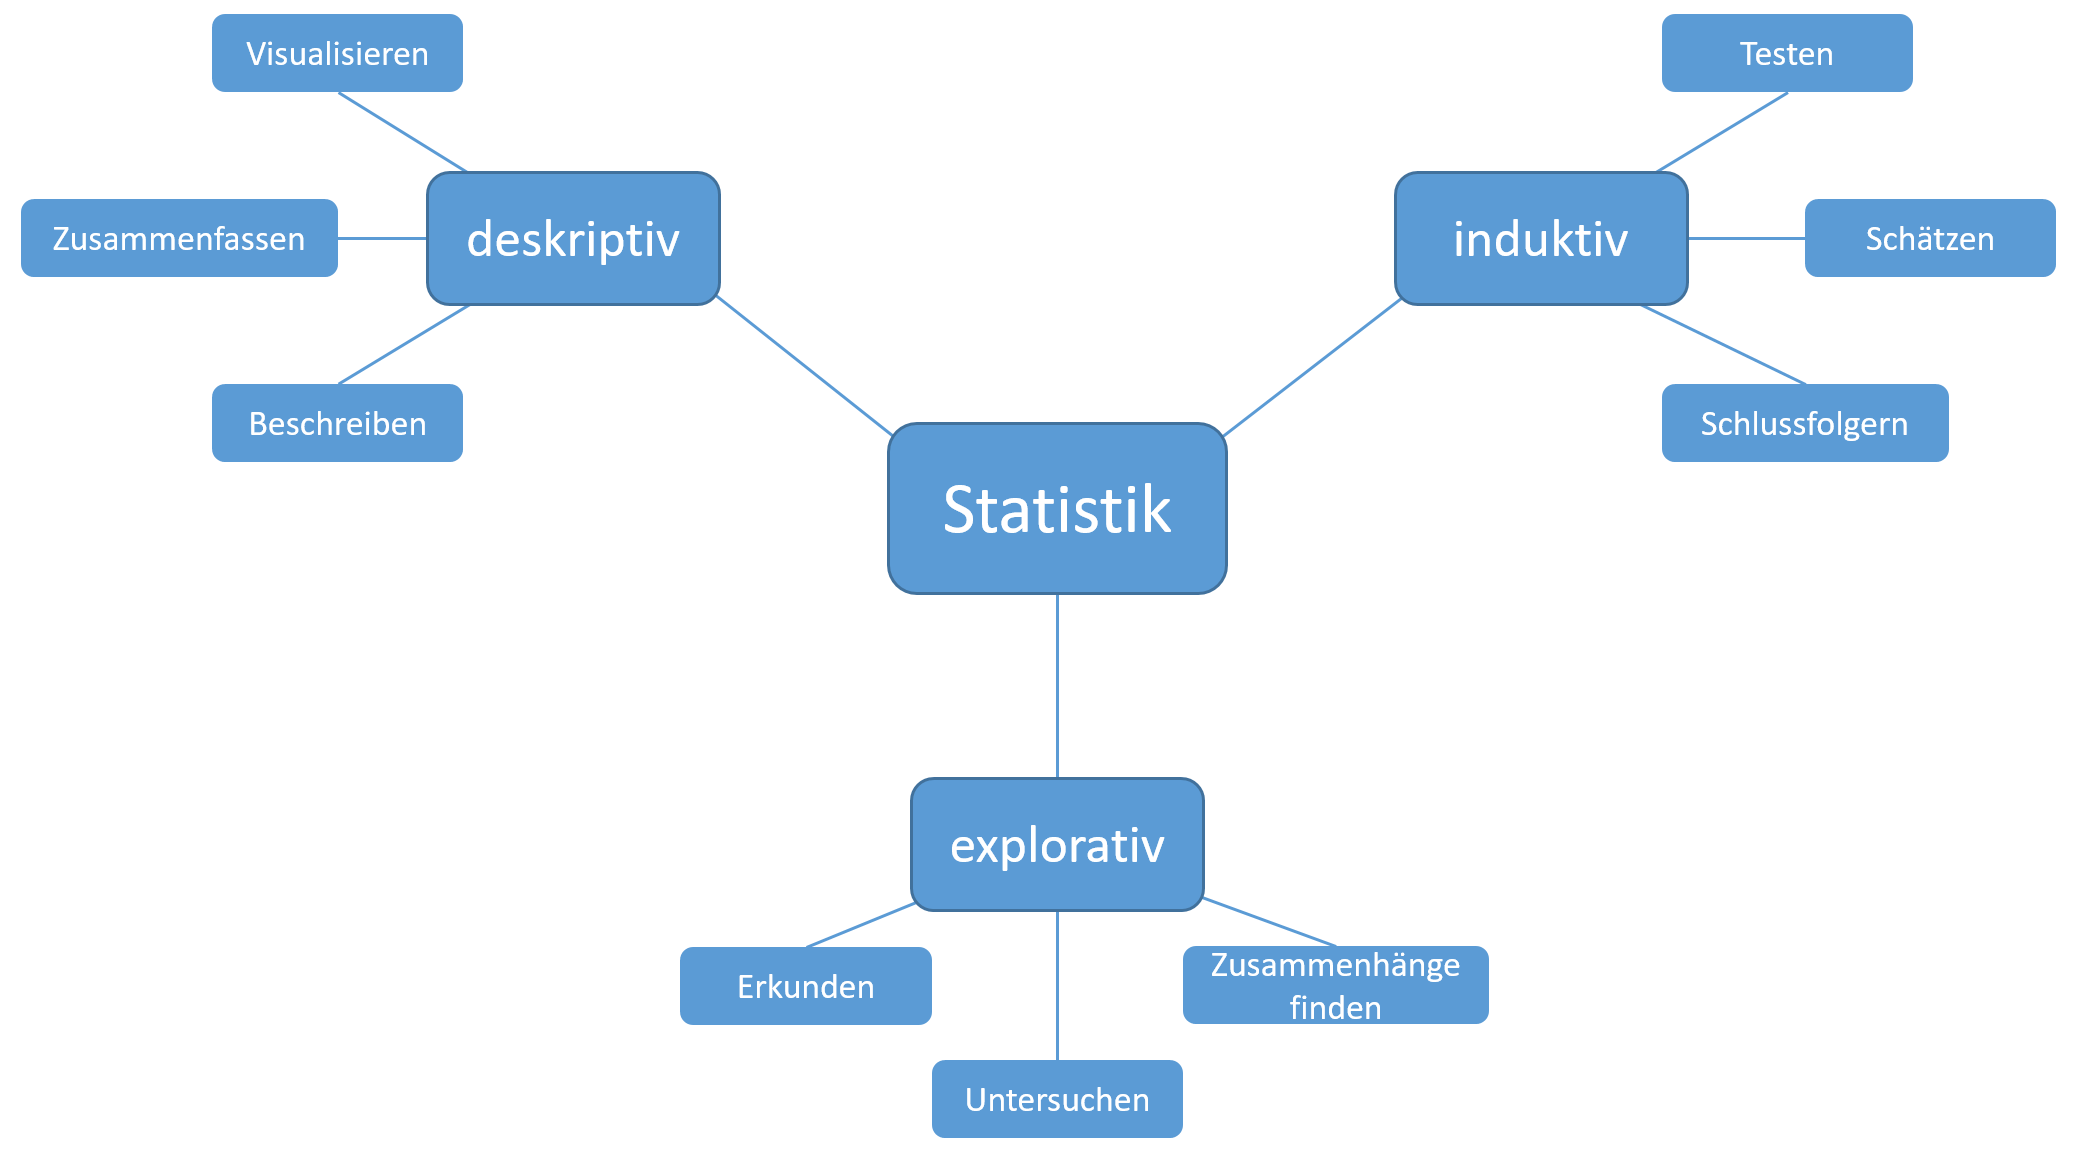
\includegraphics[scale=0.48]{images/statistik.PNG}
\end{figure}
\end{frame}
\begin{frame}
\frametitle{Wissensentdeckung in Datenbanken}
\begin{block}{Definition: Wissensentdeckung in Datenbanken}
Wissensentdeckung in Datenbanken (engl. \textit{Knowledge Discovery in Databases}, kurz KDD) ist der nicht-triviale Prozess der Identifikation gültiger, bisher unbekannter, potentiell nützlicher und letztendlich verständlicher Muster in Daten.\cite{fayyad_data_1996}
\end{block}
Anmerkungen:
        \begin{itemize}[<+->]
        	\item \textit{Daten} sind hier eine Menge von Fakten
            \item \textit{nicht-trivial} bedeutet hier, dass komplexere Vorgänge wie Suche oder Folgerungen 
(Inferenz) in Abgrenzung zu einfachen Datenbankabfragen angewendet werden
            \item das erlernte Wissen soll \textit{gültig} im Sinne der Statistik sein
            \item \textit{Muster} wird in dieser Definition allgemein und eher im Sinne von Wissen aufgefasst
        \end{itemize}
\end{frame}

\begin{frame}
\frametitle{KDD Vorgehensmodell nach Fayyad et. al.}
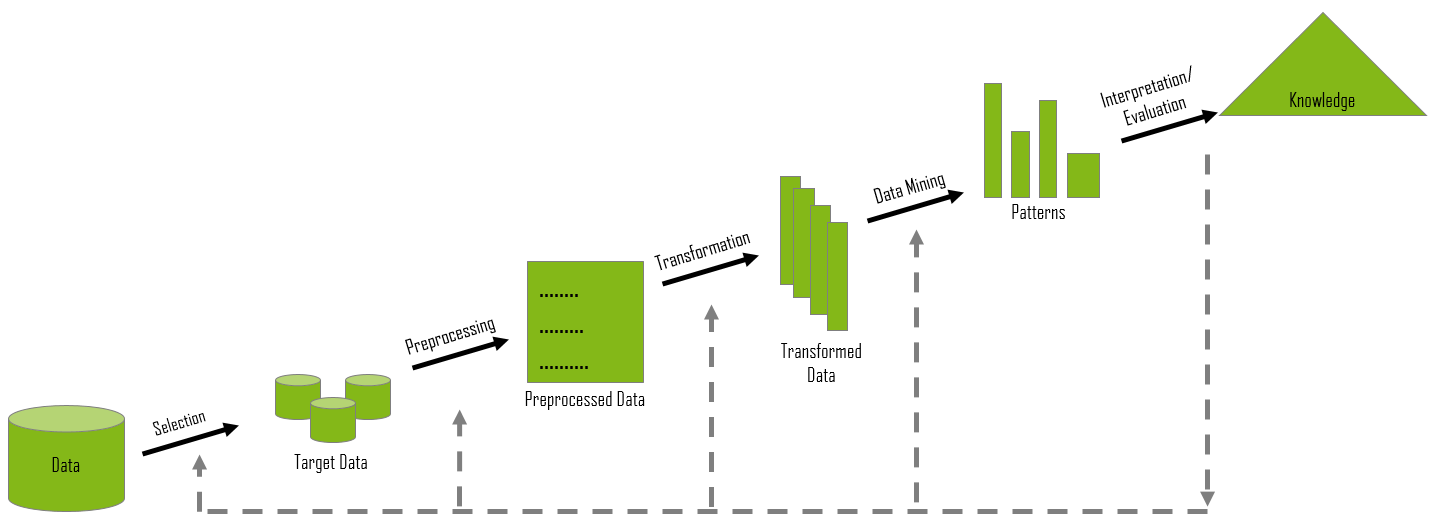
\includegraphics[scale=0.6]{images/faxxer-kdd.PNG} 
\end{frame}
\begin{frame}
\frametitle{Phasen des KDD-Vorgehensmodells}
Die einzelnen Phasen bestehen aus folgenden Inhalten:
\begin{enumerate}[<+->]
\item[0.] Zielsetzung:
\begin{itemize}[<+->]
\item Verständnis für Anwendungsgebiet aufbauen
\item Bestehendes Wissen zusammentragen
\item Ziel aus Sicht des Kunden entwickeln
\end{itemize}
\item Auswahl: Für das Ziel relevante Daten auswählen
\item Vorverarbeitung:
\begin{itemize}[<+->]
\item Entfernung von Rauschen (sofern sinnvoll) oder Informationssuche für Modellierung von Rauschen
\item Untersuchung von Ausreißern
\item Strategie für fehlende Werte festlegen
\item Betrachtung von zeitlichen Informationen und bekannten Veränderungen
\end{itemize}
\item Transformation:
\begin{itemize}[<+->]
\item Auswahl von geeigneten Merkmalen und gegebenenfalls Generierung neuer Merkmale
\item Gegebenenfalls Reduktion der Dimension
\item Auswahl geeigneter Datentypen
\end{itemize}
\end{enumerate}
\end{frame}
\begin{frame}
\begin{enumerate}[<+->]
\item[4.] Data Mining:
\begin{itemize}[<+->]
\item Bestimmung der geeigneten Data Mining Methode(n) unter Berücksichtigung des formulierten Ziels aus Schritt $0$ (Klassifikation, Regression, Clustern,...)
\item Explorative Analyse (Regressionsanalysen, Visualisierungen, ...)
\item Auswahl geeigneter Algorithmen
\item Ausführen der Algorithmen zur Mustererkennung
\end{itemize}
\item[5.] Evaluation: 
\begin{itemize}[<+->]
\item Interpretation der bisherigen Ergebnisse (gegebenenfalls Wiederholung der Schritte 0 bis 4)
\item Visualisierung der Ergebnisse
\item Ergebniserstellung
\end{itemize}
\end{enumerate}
\end{frame}

\begin{frame}
\frametitle{CRISP-DM}
\begin{figure}[hbtp]
\centering
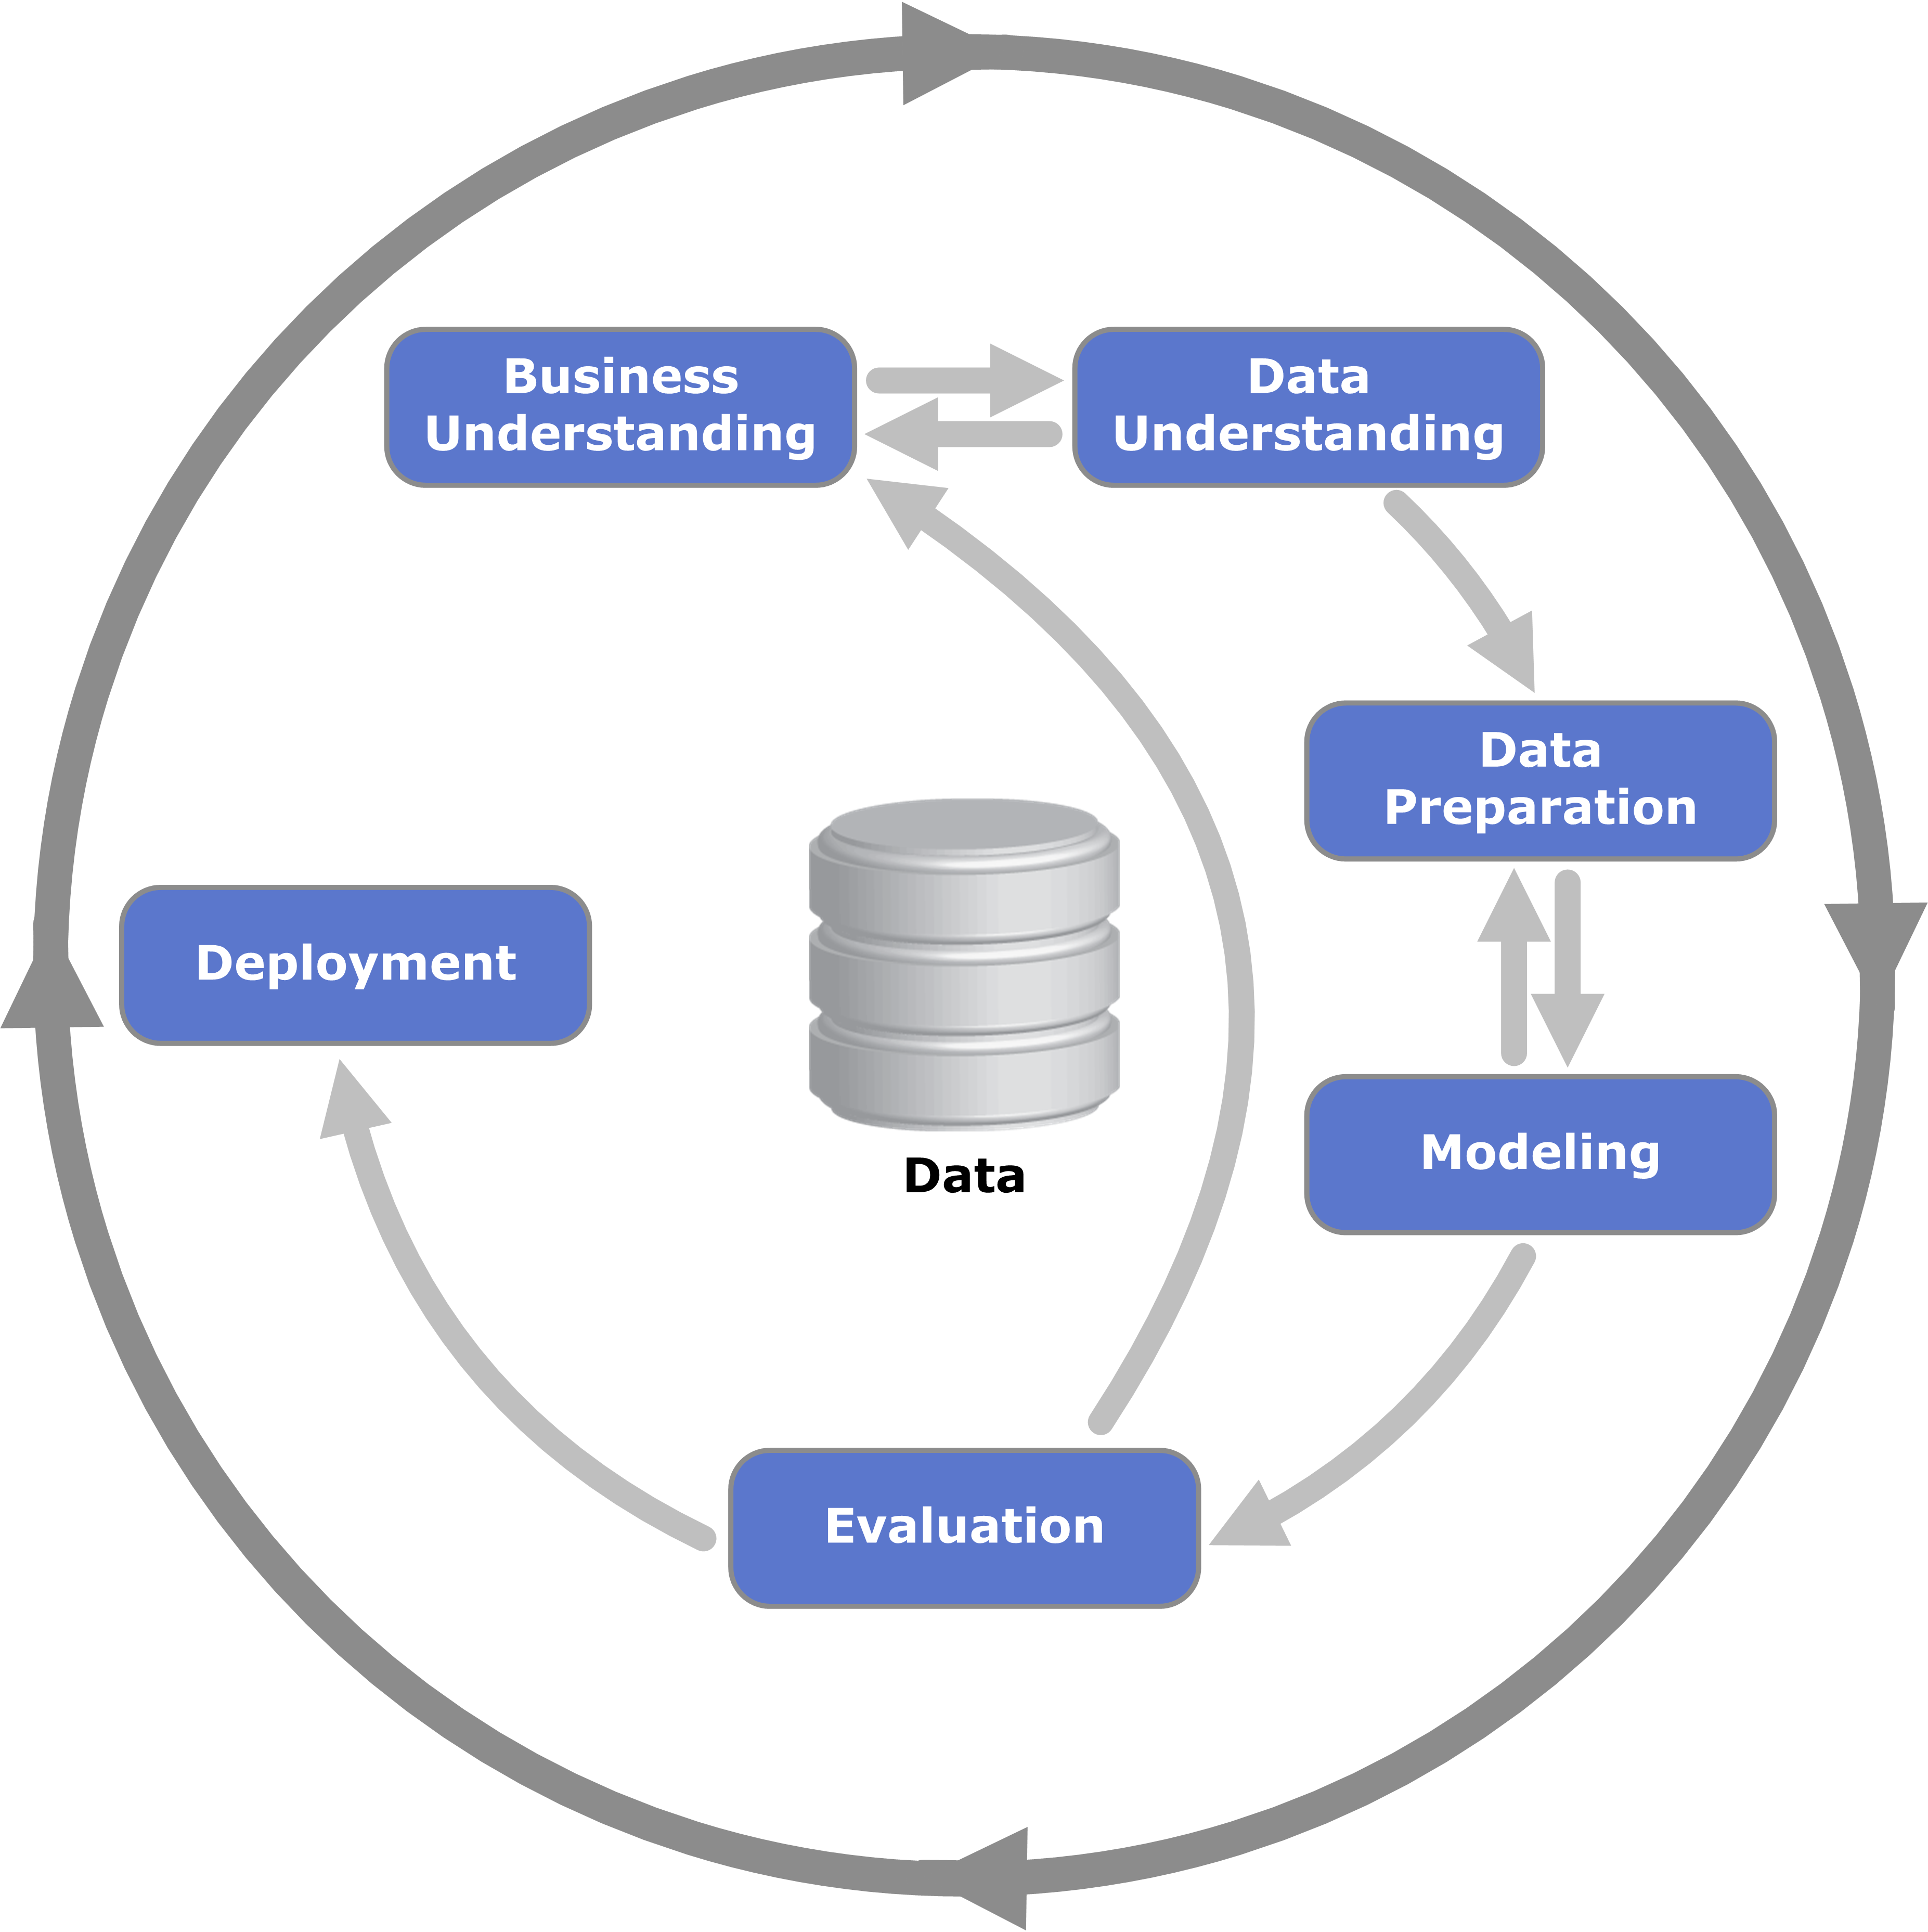
\includegraphics[scale=0.4]{images/CRISP-DM_Process_Diagram.png}
\caption{Vorgehensmodell nach CRISP-DM}
\end{figure}

\end{frame}
\begin{frame}
\frametitle{Maschinelles Lernen}
Es gibt viele verschiedene Definitionen und Beschreibungen des Gebiets des maschinellen Lernens. Zwei bekannte sind etwa:
\begin{block}{Maschinelles Lernen}
\begin{itemize}
\item \glqq [Machine learning is] the field of study that gives computers the ability to learn without explicity programmed\grqq{} -Arthur Samuel
\end{itemize}
\end{block}
\end{frame}
\begin{frame}
\centering
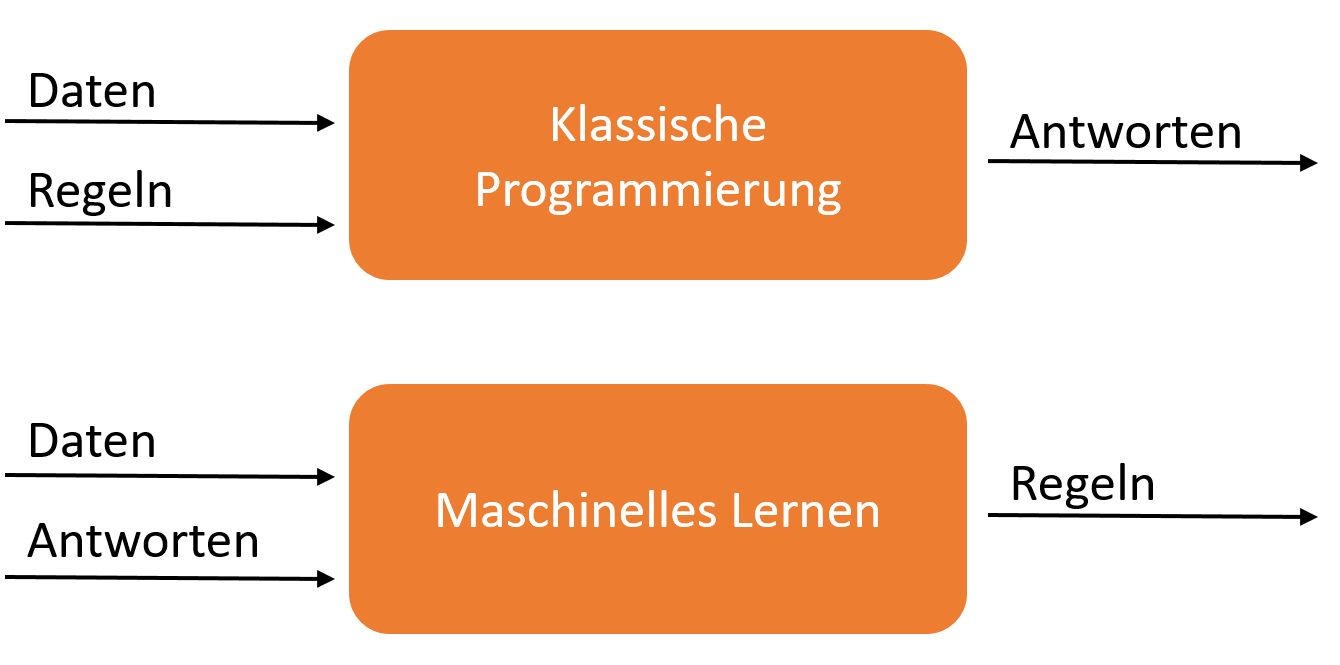
\includegraphics[scale=0.6]{images/MLparadigma.PNG} 
\end{frame}
\begin{frame}
\frametitle{Arten des maschinellen Lernens}
Die meisten Aufgaben des maschinellen Lernens lassen sich in die folgenden drei Kategorien einordnen:
\begin{enumerate}[<+->]
\item Überwachtes Lernen (engl. supervised learning):
	\begin{itemize}[<+->]
		\item Eingabewerte $x$ und Ausgabewerte $y$ sind für historische Beispiele bekannt
		\item Ziel: Funktion $f$ zu erlernen mit $f(x) = y$
		\item Für neue Eingabewerte kann somit der Ausgabewert geschätzt bzw. prognostiziert werden
	\end{itemize}
\item Unüberwachtes Lernen (engl. unsupervised learning):
	\begin{itemize}[<+->]
		\item Hier existieren nur Eingabewerte $x$, \textbf{keine} Ausgabewerte
		\item Ziel: (unbekannte) Strukturen innerhalb der Daten entdecken
	\end{itemize}
\item Verstärkendes Lernen (engl. reinforcement learning):
	\begin{itemize}[<+->]
		\item Ein (Software-) Agent kann aus mehreren Aktionen auswählen
		\item Der Agent befindet sich in einer Umgebung mit der er interagieren kann
		\item Jede gewählte Aktion überführt den Agenten in einen neuen Status innerhalb der Umgebung
		\item Der Agent erhält für jede Aktion eine Auszahlung bzw. Belohnung
		\item Ziel des Agenten ist die erhaltene (Gesamt-) Auszahlung zu maximieren
	\end{itemize}
\end{enumerate}
\end{frame}
\begin{frame}
\frametitle{Aufgabenarten des maschinellen Lernens}
Die meisten Probleme, die mit maschinellem Lernen gelöst werden sollen, lassen sich in folgende Aufgaben einteilen:
\begin{block}{Aufgaben und Ziele für maschinelles Lernen}
\begin{itemize}[<+->]
\item Klassifikation: Gegeben seien $n$ verschiedene Klassen. Jedes Objekte gehört einer dieser Klassen an. Für Objekte soll anhand ihrer Eigenschaften (features) die entsprechende Klasse prognostiziert werden. Die Zielgröße der Prognose ist hier eine nominale bzw. diskrete Größe. Insbesondere ist die wahre Klasse der Trainingsdaten bekannt.
\item Regression: Soll ein stetiger Wert prognostiziert werden, spricht man von einer Regressionsaufgabe. Der wahre Wert der Zielgröße ist für die Trainingsdaten bekannt.
\item Clusteranalyse: Verschiedene Objekte sollen zu Gruppen zusammengefasst werden, sodass die Objekte einer Gruppe möglichst ähnlich zueinander sind, und die Unterschiede zu den übrigen Gruppen möglichst groß sind. Hier existieren keine wahren Werte.
\item Dimensionsreduktion: Hochdimensionale Daten sollen in ihrer Dimension reduziert werden, sodass die Struktur möglichst erhalten bleibt.
\end{itemize}
\end{block}
\end{frame}
\begin{frame}[fragile]
\frametitle{Klassifikation}
\onslide<1->{
\begin{figure}
\begin{tikzpicture}[scale = 0.9,line cap=round,line join=round,>=triangle 45,x=1.0cm,y=1.0cm]
\begin{axis}[
x=1.0cm,y=1.0cm,
axis lines=middle,
xmin=0.0,
xmax=9.0,
ymin=0.0,
ymax=7.0,
xtick={0.0,1.0,...,9.0},
ytick={0.0,1.0,...,7.0},]
\end{axis}
\clip(0.,0.) rectangle (9.,7.);
\draw [fill=ffqqqq] (4.,2.) circle (2.5pt);
\draw [fill=ududff] (5.,4.) circle (2.5pt);
\draw [fill=ududff] (5.,6.) circle (2.5pt);
\draw [fill=ududff] (6.,5.) circle (2.5pt);
\draw [fill=ududff] (8.,5.) circle (2.5pt);
\draw [fill=ududff] (8.,6.5) circle (2.5pt);
\draw [fill=ffqqqq] (2.,2.) circle (2.5pt);
\draw [fill=ffqqqq] (2.,3.) circle (2.5pt);
\draw [fill=ffqqqq] (1.3,4.) circle (2.5pt);
\draw [fill=ududff] (5.5,3.) circle (2.5pt);
\draw [fill=ffqqqq] (3.,1.) circle (2.5pt);
\onslide<2->{
\node[circle,fill=black,inner sep=0pt,minimum size=5pt,label=below:{?}] (a) at (1.6,1.) {};
%\draw [fill=black] (5.,3.) circle (2.5pt);
}
\onslide<3->{
\node[circle,fill=black,inner sep=0pt,minimum size=5pt,label=below:{?}] (a) at (4.,6.5) {};
}
\end{tikzpicture}
\end{figure}
}
\end{frame}
\begin{frame}
\frametitle{Regression}
\centering
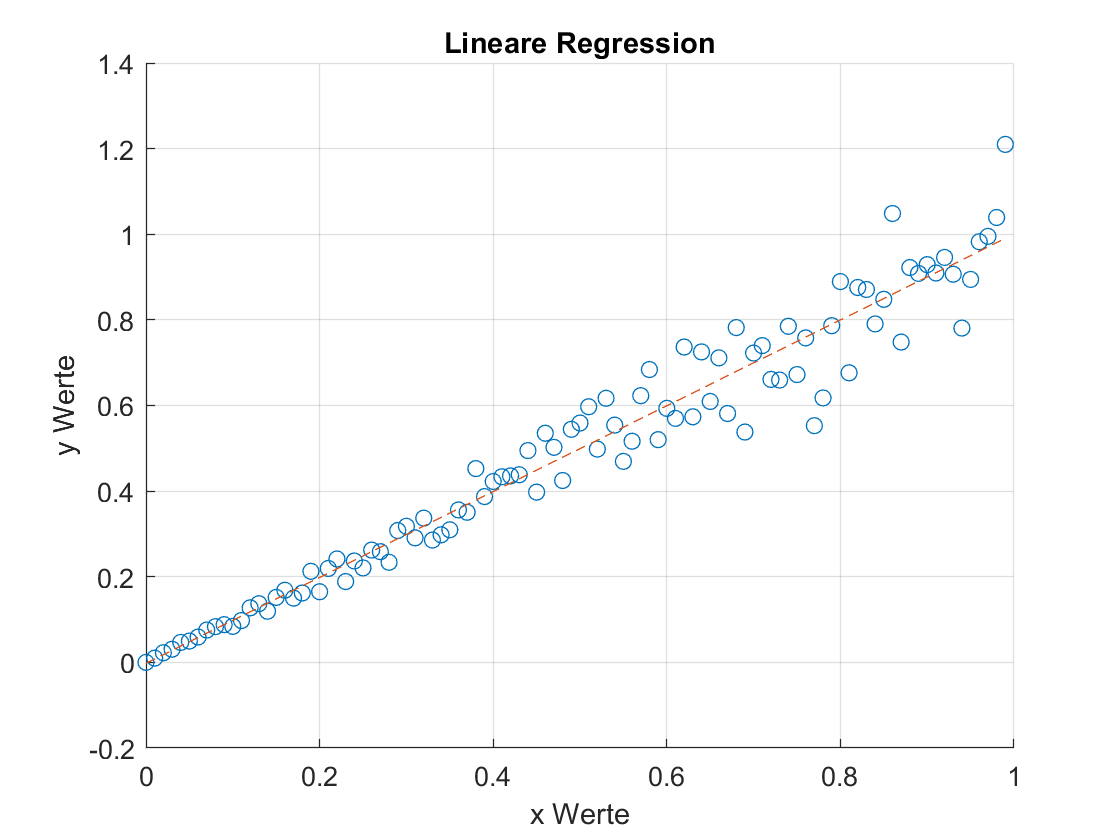
\includegraphics[scale=0.31]{images/plot_linreg.png} 
\end{frame}
\begin{frame}
\frametitle{Clusteranalyse}
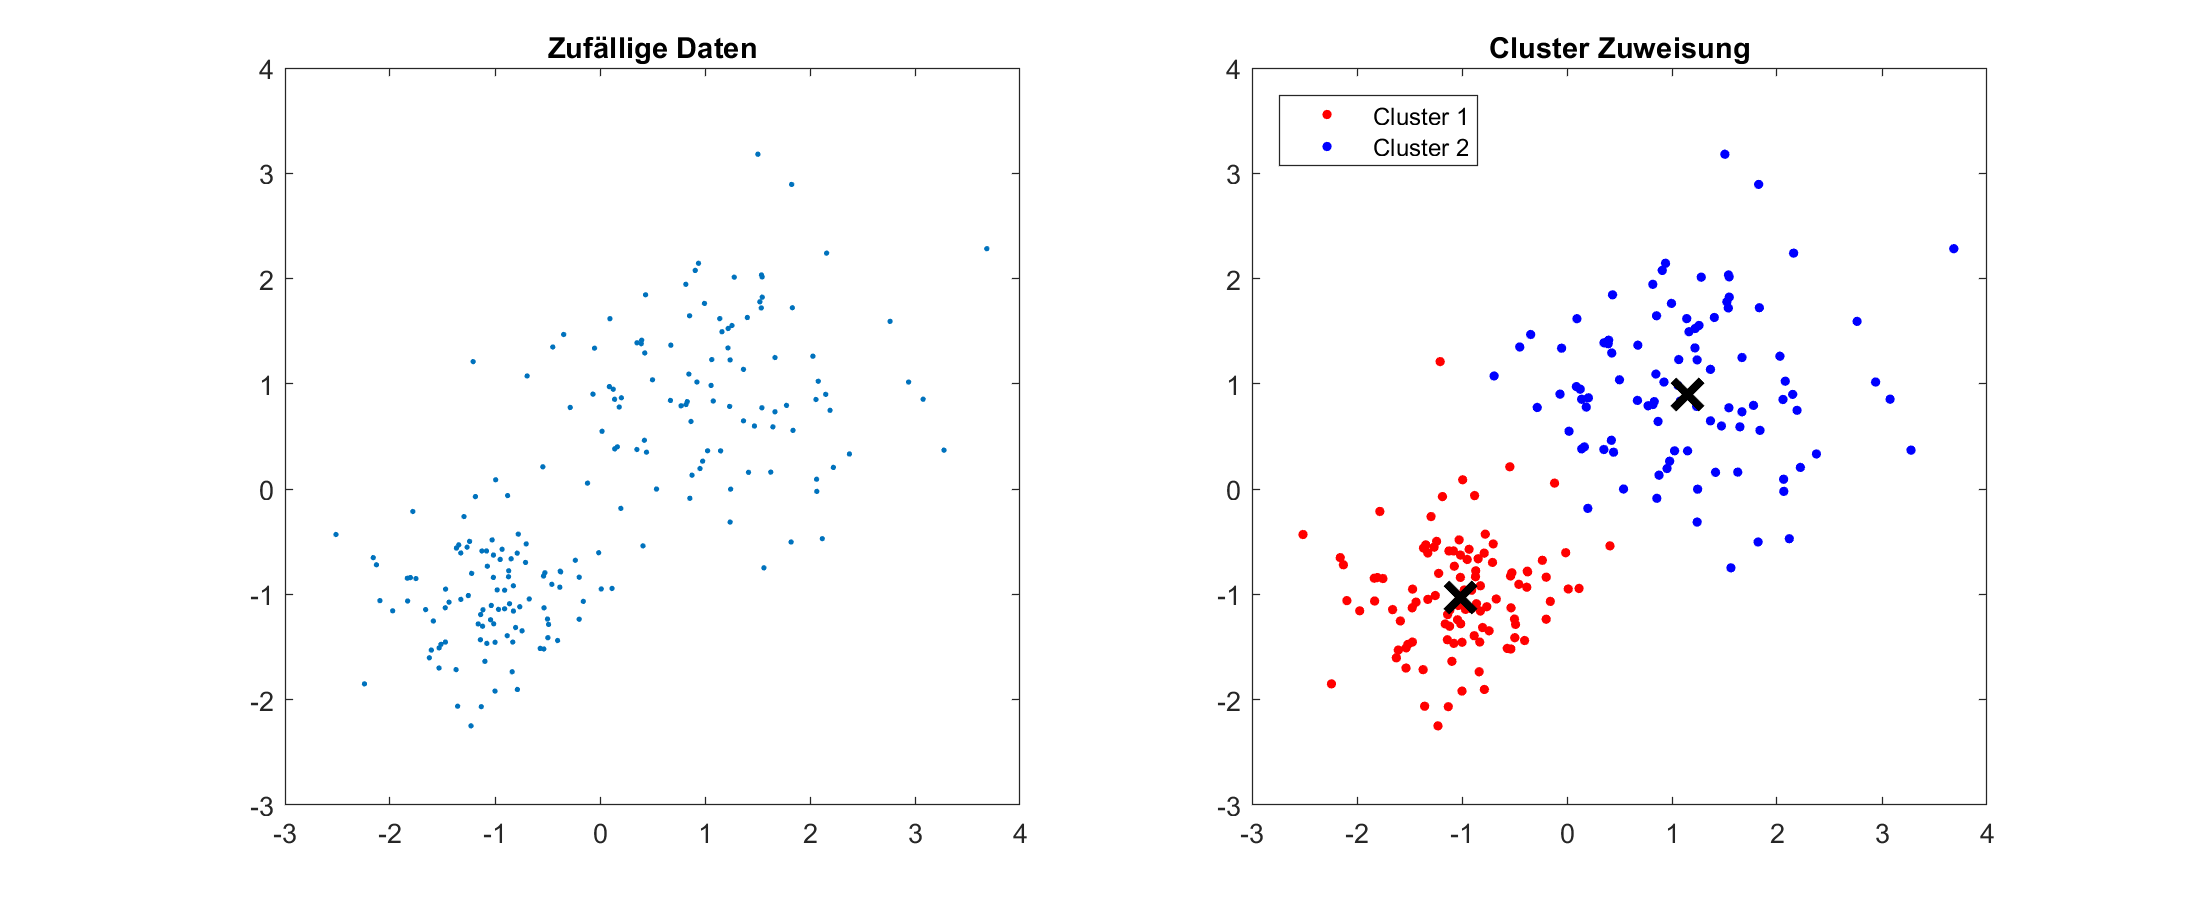
\includegraphics[scale=0.25]{images/cluster_plot.png} 
\end{frame}
\begin{frame}
\frametitle{Die Lineare Regression}
Als ein erstes, einfaches und bekanntes Verfahren, soll hier die lineare Regression behandelt werden.
\pause
\begin{itemize}[<+->]
\item Dazu seien folgende Beispielwerte gegeben:\\
\begin{tabular}{c|c}
Eingabe $x$ & Ausgabe $y$\\
\hline
$0$ & $0$\\
$1$ & $0$\\
$2$ & $1.5$\\
$3$ & $2$\\
\end{tabular}
\item Wir wollen den Zusammenhang zwischen $x$ und $y$ durch eine lineare Funktion modellieren, d.h.
\[ h_\theta (x) = \theta_0 + \theta_1\cdot x = \hat{y} \]
\item $h_\theta$ ist die sog. Hypothese (mit Parameter $\theta = (\theta_0,\theta_1)$
\item $\hat{y}$ ist der geschätzte Wert von $y$ (auf Grundlage von $h_\theta$)
\item Eine mögliche Hypothese ist etwa $h_\theta(x) = 1 - x$
\end{itemize} 
\end{frame}
\begin{frame}
\begin{itemize}[<+->]
\item Die Hypothese $h_\theta(x) = 1 - x $ führt zu folgenden Prognosen für $y$:\\[0.1cm]
\begin{tabular}{c|c|c|c}
Eingabe $x$ & Prognose $\hat{y}$ & Wahre Ausgabe $y$ & Differenz $\vert y - \hat{y}\vert$ \\ 
\hline 
$0$ & $1$ & $0$ & $1$ \\ 
$1$ & $0$ & $0$ & $0$ \\ 
$2$ & $-1$ & $1.5$ & $2.5$ \\  
$3$ & $-2$ & $2$ & $4$ \\  
\end{tabular}
\item Offensichtlich liefert diese Hypothese keine annehmbaren Prognosen, da die Fehler groß sind
\item Gesucht sind also Werte für $\theta_0$ und $\theta_1$ die \glqq am besten\grqq{} zu den Daten passen
\item Zunächst muss festgelegt werden, wie der Abstand zwischen der Hypothese und den wahren Ausgaben gemessen werden soll
\item Dafür verwenden wir eine sogenannte Kostenfunktion $L$
\item Für die lineare Regression ist der mittlere quadratische Fehler aus theoretischen Gründen gut geeignet:
\[ L(\theta_0,\theta_1) = \frac{1}{n}\sum_{i=1}^n (\hat{y}_i - y_i)^2 \]
\end{itemize}
\end{frame}
\begin{frame}
\begin{itemize}[<+->]
\item Lösen des Optimierungsproblems 
\[ \min\limits_{\theta_0,\theta_1} L(\theta_0,\theta_1) \]
liefert also die \glqq besten\grqq{} Parameter, in dem Sinne, dass hier ein minimaler Fehler bezüglich der gewählten Kostenfunktion und der gewählten Hypothese (hier linear) erzeugt wird
\item Für den mittleren quadratischen Fehler als Kostenfunktion, kann im Falle der linearen Regression eine analytische Lösung angegeben werden\footnote{Unter bestimmten formalen Annahmen, wie etwa standardnormalverteilten Fehlertermen}
\begin{align*}
\theta_1 &= \frac{\sum_{i=1}^n (x_i - \bar{x})(y_i - \bar{y})}{\sum_{i=1}^n (x-\bar{x})^2}\\
\theta_0 &= \bar{y} - \theta_1\cdot \bar{x}
\end{align*}
\item Alternativ kann das obige Minimierungsproblem mit Methoden der Optimierung (häufig Gradientenabstieg) gelößt werden
\end{itemize}
\end{frame}
\begin{frame}
\begin{itemize}[<+->]
\item Doch Vorsicht: Es sollten \textbf{nie} alle Daten zum bestimmen der Parameter verwendet werden
\item Andernfalls kann die Genauigkeit der Hypothese nicht evaluiert werden
\item Und die so gefundenen Parameter sind meistens zu stark an die Daten angepasst
\item Das Ermitteln der Parameter wird \textit{Training} genannt
\item Um die Hypothese beurteilen zu können, werden die Daten in ein Trainings- und Testdatensatz aufgeteilt
\end{itemize}
\end{frame}
\begin{frame}
Folgende Notation wird von nun an verwendet:
\begin{itemize}
\item $N$ ist die Anzahl aller Datenpunkte bzw. Beispiele, $K$ ist die Anzahl der Attribute eines jeden Beispiels
\item $x_{i,k}$ ist der Wert des $i$-ten Beispiels/Datenpunktes vom $k$-ten Attribut
\item $X_i$ ist der Vektor $(x_{i,1},\ldots,x_{i,N})$
\item $X$ ist die Matrix 
\[
\begin{pmatrix}
1 & x_{1,1} & x_{1,2} & \cdots & x_{1,K} \\
1 & x_{2,1} & x_{2,2} & \cdots & x_{2,K} \\
\vdots &\vdots & \vdots & \ddots & \vdots \\
1 & x_{N,1} & x_{N,2} & \cdots & x_{N,K}\\
\end{pmatrix}
\]
\item $y_i$ ist der Zielwert des $i$-ten Beispiels
\item $Y$ ist der Vektor $(y_1,\ldots,y_N)$
\end{itemize}
\end{frame}
\begin{frame}
\frametitle{Residuenplots}
Eine weitere, sehr hilfreiche Möglichkeit, das gelernte Modell zu evaluieren ist ein Plot der Residuen.
\begin{itemize}[<+->]
\item Ein Residuum ist die Differenz von wahrem und prognostiziertem Wert, d.h. 
\[ r = y – \hat{y} \]
\item Anschließend wird die Verteilung der Residuen dargestellt und der Verlauf der Residuen gezeichnet
\item Im Idealfall liegen die meisten Residuen nahe der $0$ und es gibt nur wenige Ausreißer, optisch erinnert die Verteilung der Residuen einer Gaußglocke
\item Oftmals lassen sich systematische Fehler feststellen, wie 
\begin{itemize}[<+->]
\item viel mehr positive als negative Residuen, 
\item periodischer Wechsel zwischen positiven und negativen Residuen, 
\item Gleichverteilung der Residuen,
\item ...
\end{itemize}
\end{itemize}
\end{frame}
\begin{frame}
\frametitle{Trainings- und Testmenge}
Um die Performance eines Klassifikators oder eine Regression zu evaluieren, wird die Datenmenge in eine Trainings- und in eine Testmenge aufgeteilt
\begin{itemize}[<+->]
\item Seien $(X_1,y_1),(X_2,y_2),\ldots,(X_{n+m},y_{n+m})$ alle Datenpunkte/Instanzen
\item Die Instanzen $(X_1,y_1),\ldots,(X_n,y_n)$ werden für das Trainieren, also das Spezifizieren des Klassifikators verwendet
\item Die übrigen $m$ Instanzen $(X_{n+1},y_{n+1}),\ldots,(X_{n+m},y_{m+n})$ werden \textbf{nicht} für das Trainieren verwendet sondern bilden die Testmenge
\item Um die Performance des Modells zu evaluieren, wird das Modell auf die Testmenge angewendet, also Instanzen die das Modell bisher nicht gesehen hat
\item Da die Lösungen $y_i$ bekannt sind, kann so das Modell geprüft werden
\item Die Aufteilung in Trainings- und Testmenge sollte immer zufällig durchgeführt werden (außer bei zeitabhängigen Instanzen!)
\item Üblicherweise werden $60\%$ der Instanzen für das Trainieren und $40\%$ für das Testen verwendet
\item Bei sehr großen Datenmengen können auch $90\%$ für das Trainieren und die übrigen $10\%$ für das Testen verwendet werden
\end{itemize}
\end{frame}
\begin{frame}
\frametitle{Validierungsdatensatz}
\begin{itemize}[<+->]
\item Der Trainingsfehler $L_{Training}$ist der Fehler nach der Kostenfunktion bezüglich der Trainingsmenge
\item Der Testfehler $L_{Test}$ ist der Fehler nach der Kostenfunktion bezüglich der Testmenge
\item Sollen Hyperparameter, also Freiheitsgrade des Modells, oder verschiedene Hypothesen verglichen werden, so darf das \textbf{nicht} mittels des Testfehlers geschehen
\item Statt die Daten nur in Trainings- und Testdaten aufzuteilen, werden die Daten in Trainings-, Validierungs- und Testdaten aufgeteilt
\item Eine übliche Aufteilung ist $60\%$ Trainings-, $20\%$ Validierungs- und $20\%$ Testdaten
\item Der Validierungsfehler $L_{Val}$ ist der Fehler nach der Kostenfunktion bezüglich der Validierungsmenge
\item Der Vergleich verschiedener Hyperparameter oder Hypothesen erfolgt dann über den Validierungsfehler
\end{itemize}
\end{frame}
\begin{frame}
\frametitle{Über- und Unteranpassung}
Ein auf maschinellem Lernen basierendes Modell muss gut evaluiert werden. Zwei häufige Probleme sind Über- und Unteranpassung.
\begin{block}{Über- und Unteranpassung}
\begin{itemize}[<+->]
\item Überanpassung (engl. overfitting): Ein Modell ist \textit{überangepasst}, wenn es zu stark mit den Daten zusammenhängt und somit auch das Rauschen der Daten mitberücksichtigt. Das Modell enthält zu viele Freiheitsgrade, die nicht durch die Daten begründet werden können.

\item Unteranpassung (engl. underfitting): Ein Modell ist \textit{unterangepasst}, wenn es den Trend der zugrundeliegenden Daten nicht passend abbilden kann und die Daten nicht ausreichend beachtet. Dies kann etwa an zu wenigen Daten, oder einem nicht passenden Modell liegen (etwa ein lineares Modell für einen nicht-linearen Verlauf)
\end{itemize}
\end{block}
\end{frame}
\begin{frame}
\frametitle{Über- und Unteranpassung}
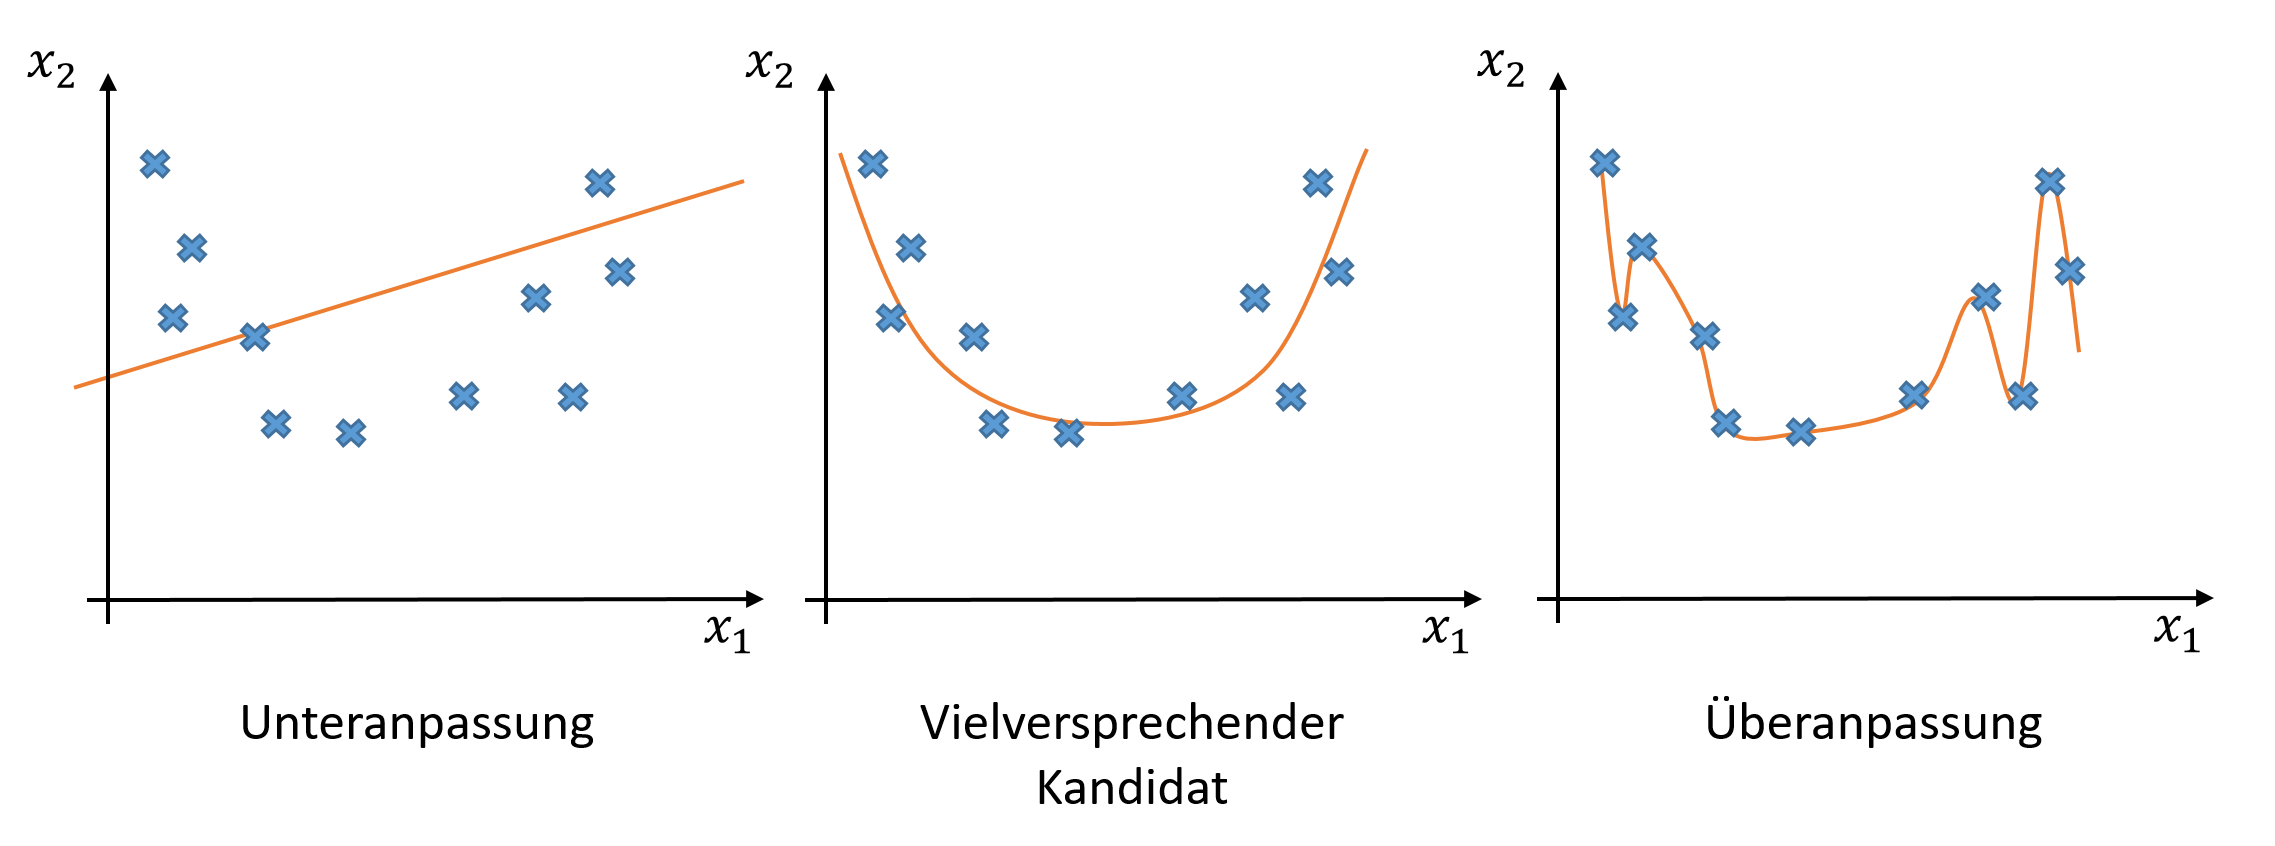
\includegraphics[scale=0.5]{images/over_under_fitting.PNG} 
\end{frame}
\begin{frame}
\frametitle{Einfache Kreuzvalidierung}
Um ungünstige Aaufteilungen in Trainings- und Testmenge zu vermeiden, kann dieses mehrfach wiederholt werden:
\begin{itemize}[<+->]
\item Sei $T$ die Menge der zur Verfügung stehenden Datenpunkte, mit $|T| = N$
\item $T$ wird in $k\leq N$ (möglichst) gleich große disjunkte Teilmengen $T_1,T_2,\ldots,T_k$ aufgeteilt
\item Für $i = 1 \text{ bis } k$:
\begin{enumerate}[<+->]
\item Wähle $T_i$ als Testmenge (auch Kreuzvalidierungsmenge)
\item Wähle $T \setminus T_i$ als Trainingsmenge
\item Trainiere das gewählte Modell mit der Trainingsmenge aus Schritt 2 und der Kreuzvalidierungsmenge aus Schritt 1
\item Bestimme den Trainings- und den Kreuzvalidierungsfehler
\end{enumerate}
\item Der Gesamte Fehler ist das arithmetische Mittel der einzelnen Fehler 
\end{itemize}
\end{frame}
\begin{frame}
\frametitle{Über- und Unteranpassung graphisch identifizieren}
\centering
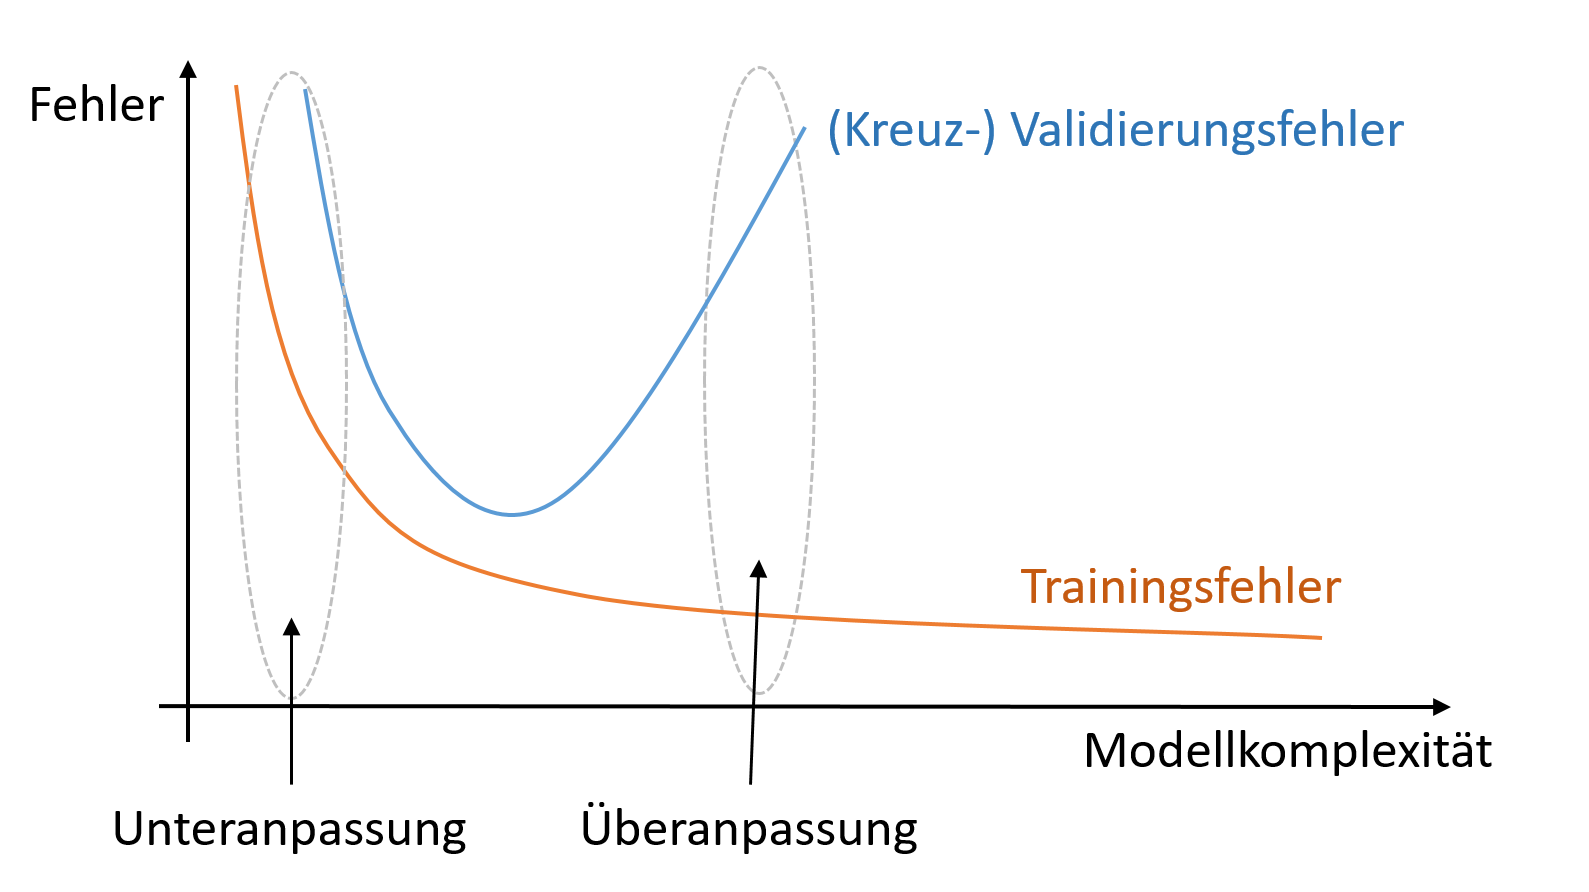
\includegraphics[scale=0.4]{images/under-over-fitting2.PNG} 
\end{frame}
% KNN Algorithmus
\begin{frame}
\frametitle{kNN-Algorithmus}
Hier wird nur die binäre Klassifikation betrachtet, d.h. es gibt zwei mögliche Klassen: $0$ und $1$\\[0.2cm]
Kommen wir nun zum ersten Algorithmus zur Klassifikation.
\begin{block}{kNN}
Der kNN-Algorithmus (k-nearest-neighbors) ist ein Klassifikations-Algorithmus, der für einen neuen Punkt $x$ mit Hilfe von $k\in\mathbb{N}$ Trainingsbeispielen, die am nächsten an $x$ liegen, die Klasse von $x$ vorhersagt.
\end{block}
\pause
Diese Beschreibung lässt einige Fragen offen:
\begin{itemize}
\item Wie wird bestimmt, welche Punkte \glqq am nächsten\grqq{} liegen?
\item Wie wird auf Grundlage der $k$ Punkte bestimmt, welche Klasse $x$ zugeordnet wird?
\item Wie wird $k$ gewählt?
\end{itemize}
\end{frame}
\begin{frame}[fragile]
\begin{figure}
\begin{tikzpicture}[scale = 0.9,line cap=round,line join=round,>=triangle 45,x=1.0cm,y=1.0cm]
\begin{axis}[
x=1.0cm,y=1.0cm,
axis lines=middle,
xmin=0.0,
xmax=9.0,
ymin=0.0,
ymax=7.0,
xtick={0.0,1.0,...,9.0},
ytick={0.0,1.0,...,7.0},]
\end{axis}
\clip(0.,0.) rectangle (9.,7.);
\draw [line width=2.pt,color=wqwqwq] (5.,3.) circle (2.cm);
\draw [fill=black] (5.,3.) circle (2.5pt);
\draw [color=black] (5.,3.) node {x};
\draw [fill=ffqqqq] (4.,2.) circle (2.5pt);
\draw [fill=ududff] (5.,4.) circle (2.5pt);
\draw [fill=ududff] (5.,6.) circle (2.5pt);
\draw [fill=ududff] (6.,5.) circle (2.5pt);
\draw [fill=ududff] (8.,5.) circle (2.5pt);
\draw [fill=ududff] (8.,6.5) circle (2.5pt);
\draw [fill=ffqqqq] (2.,2.) circle (2.5pt);
\draw [fill=ffqqqq] (2.,3.) circle (2.5pt);
\draw [fill=ffqqqq] (2.,4.) circle (2.5pt);
\draw [fill=ududff] (5.5,3.) circle (2.5pt);
\draw [fill=ffqqqq] (3.,1.) circle (2.5pt);
\end{tikzpicture}
\caption{\begin{small} Nachbarschaft bzgl. des euklidischen Abstandes des Punktes $(5,3)$ für $k=3$\end{small}}
\end{figure}
\end{frame}
\begin{frame}[fragile]
\frametitle{Vorgehen für kNN}
%Bevor diese drei Fragen behandelt werden, wird zunächst das allgemeine Vorgehen von kNN vorgestellt:\\[0.2cm]
\begin{algorithm}[H]
 \Parameters{$k$, Norm}\\
 \KwData{Traingingsdaten $(x_i,y_i) , i = 1,\ldots,m$\\ 
 $~~~~~~~~~$ Testdaten $(x_i,y_i) , i = m+1,\ldots,m+n$}
 \KwResult{Vorhergesagte Klassen $\hat{y}_i$ für $i=m+1,\ldots,m+n$ }
 \For{Jeden Datenpunkt $x_i$ der Trainingsdaten}{
 	Bestimme die $k$ Punkte aus der Trainingsmenge, die bzgl. der gewählten Norm am nächsten an $x_i$ liegen\\
	Die Prognostizierte Klasse $\hat{y}_i$ ist die Klasse, die am häufigsten unter diesen $k$ Punkten vorkommt
 }
 \Return $[\hat{y}_{m+1},\ldots,\hat{y}_{m+n}]$
\end{algorithm}
\begin{itemize}[<+->]
\item Der Algorithmus wird also maßgeblich durch die konkreten Wahl der Norm und $k$ bestimmt
\item Statt einfach die Mehrheit zu nehmen, kann auch die Entfernung der Nachbarpunkte mit in die Wertung einbezogen werden
\item $k$ wird häufig ungerade gewählt, um einen Gleichstand zu vermeiden
\end{itemize}
\end{frame}
\begin{frame}
    \begin{columns}[T]
        \begin{column}{0.49\textwidth}
        	Für das Distanzmaß existiert eine Vielzahl von Möglichkeiten, einige bekannte sind etwa:
            \begin{itemize}
				\item Euklidische Norm: dist$(x,y) = \sqrt{\sum_{i} (x_i - y_i)^2}$
				\item Manhatten Metrik: dist$(x,y) = \sum_i \vert x_i-y_i \vert$
				\item Maximumsnorm: dist$(x,y) = \max_i \vert x_i - y_i \vert$
				%\item Hamming-Abstand: dist$(x,y) = \vert \lbrace i \in \lbrace1,\ldots,n\rbrace | x_i \neq y_i \rbrace$ für zwei gleichlange Wörter $x$ und $y$ 
\end{itemize}
Als Kostenfunktion kann etwa die Anzahl der falsch klassifizierten Punkte herangezogen werden.
        \end{column}
        \begin{column}{0.49\textwidth}
            \begin{figure}[hbtp]
				\centering
					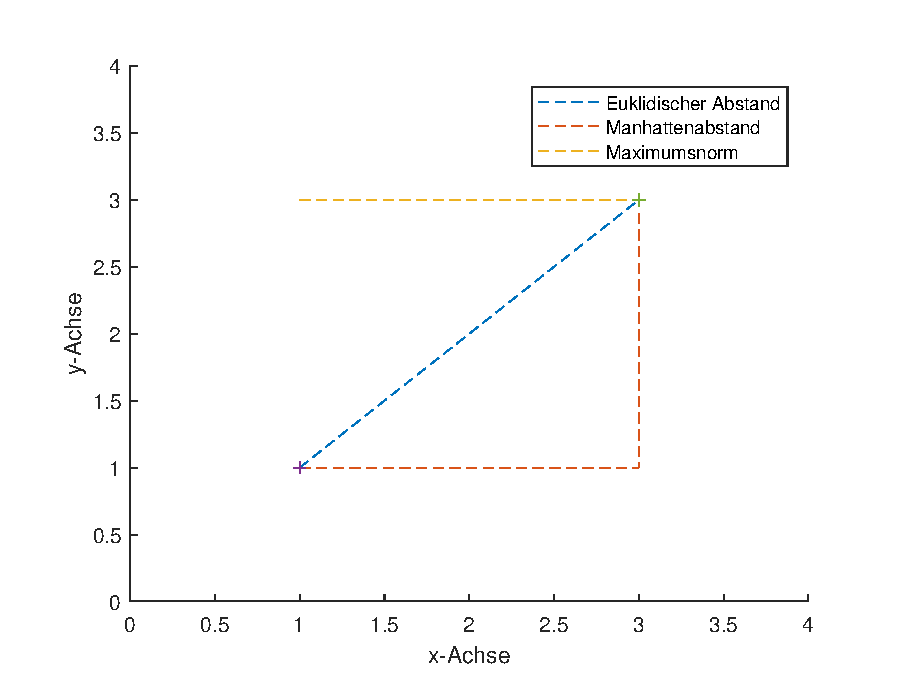
\includegraphics[scale=0.4]{images/plot_distances.eps}
				\caption{Visualisierung der verschiedenen Abstandsmaße}
			\end{figure}
        \end{column}
    \end{columns}
\end{frame}
\begin{frame}
\frametitle{Wahl von $k$ -- Die Ellbogen Methode}
\centering
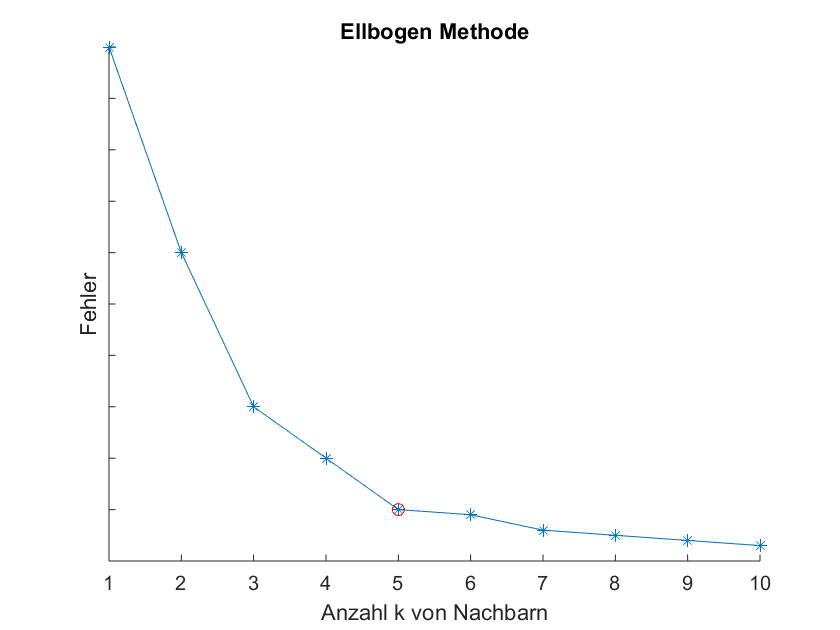
\includegraphics[scale=0.4]{images/plot_elbow.png} 
\end{frame}
\begin{frame}
\begin{itemize}[<+->]
\item Für verschiedene Werte von $k$ wird die Performance des Klassifikators evaluiert, indem der Validierungsfehler ermittelt wird
\item In einem Plot werden die Werte von $k$ gegen die dazugehörigen Validierungsfehler aufgetragen
\item Visuell wird nun der \glqq Knick\grqq{} in dem Verlauf ermittelt
\item Da der Graph häufig wie ein geknickter Arm und der Knick-Punkt wie ein Ellbogen, wird die Methode als Ellbogen Methode bezeichnet
\item In einigen Fällen kann ein eindeutiger Knick-Punkt ermittelt werden
\end{itemize}
\end{frame}
\begin{frame}
\frametitle{Die logistische Regression}
\begin{columns}[T]
        \begin{column}{0.49\textwidth}
        	\vspace{0.5cm}Bevor der eigentliche Algorithmus behandelt wird, betrachten wir zunächst die sogenannte Sigmoid Funktion:
				\begin{equation*}
					\text{sigmoid}(x) = \frac{1}{1+\exp(-x)}
				\end{equation*}
			Unter Sigmoid Funktionen fallen mehrere Funktionen. In der Regel wird mit \textit{der} Sigmoid Funktion üblicherweise die obenstehende Funktion 				bezeichnet, die auch als \textit{logistische Funktion} bekannt ist
        \end{column}
        \begin{column}{0.49\textwidth}
            \begin{figure}[hbtp]
				\centering
				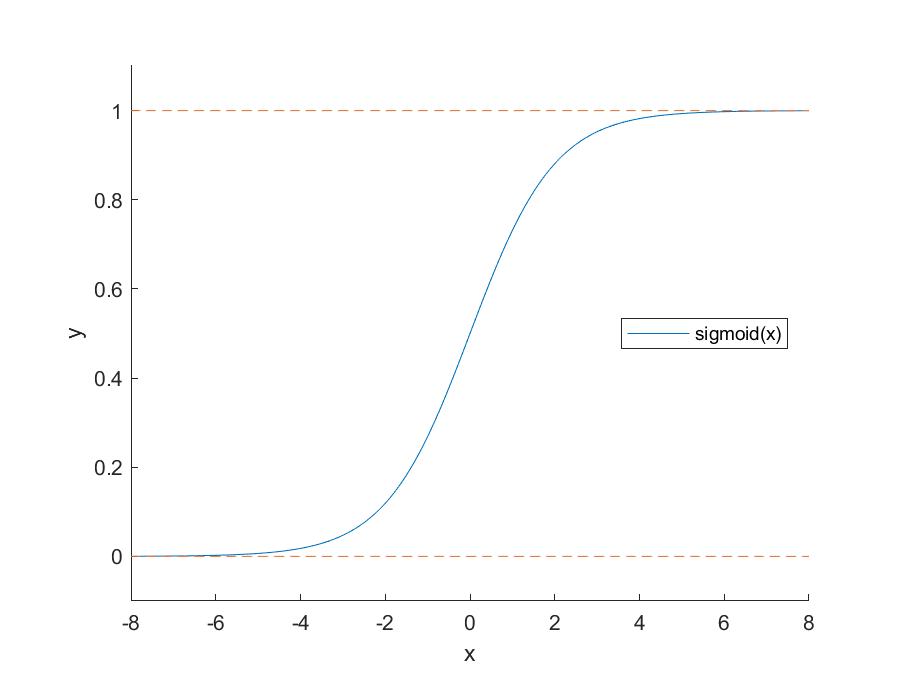
\includegraphics[scale=0.5]{images/plot_sigmoid.eps}
				\caption{Verlauf der Sigmoid-Funktion}
			\end{figure}
        \end{column}
    \end{columns}
\end{frame}
\begin{frame}
Wir betrachten zunächst eine Klassifikation mit zwei Klassen, repräsentiert durch $0$ und $1$.
\begin{itemize}
\item Zunächst sollen die Klassen durch eine lineare Funktion getrennt werden, d.h. $h_\theta(x) = \theta^T x$
\item Der Klassifikator ist \[
S_h(x):=\text{sigmoid}(h_\theta(x)) = \frac{1}{1+\exp(-h_\theta(x))} \]
\item Ist $S_h(x)\geq 0.5$, so ist die prognostizierte Klasse $1$ andernfalls $0$
\item Wann gilt $S_h(x) \geq 0.5$ ?
\begin{align*}
&S_h(x) \geq 0.5\\
\Leftrightarrow\quad &\frac{1}{1+\exp(-h_\theta(x))} \geq 0.5\\
\Leftrightarrow\quad & 0\leq h_\theta(x)
\end{align*}
\item Das heißt, alles oberhalb der Geraden $h_\theta$ wird der Klasse $1$ zugeordnet, alles unterhalb der Geraden der Klasse $0$
\item $h_\theta$ kann auch andere geeignete Formen annehmen, etwa Polynome vom Grad $n$
\end{itemize}
\end{frame}
\begin{frame}
\frametitle{Entscheidungsgrenze}
\begin{figure}[hbtp]
\centering
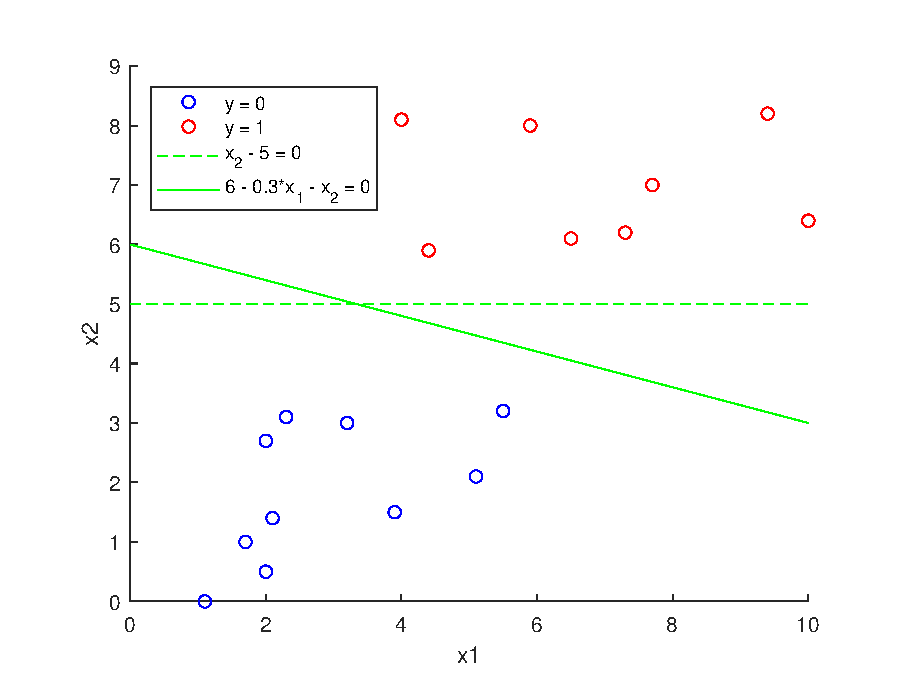
\includegraphics[scale=0.5]{images/plot_logreg.eps}
\caption{Beispiel für zwei Entscheidungsgrenzen bei logistischer Regression}
\end{figure}

\end{frame}
\begin{frame}
Wie finden wir eine gute Hypothese bzw. eine gute Entscheidungsgrenze?
\begin{itemize}[<+->]
\item Es soll die Klasse $y$ prognostiziert werden, die bei der Beobachtung x und den gegebenen Werten von $\theta$ am wahrscheinlichsten sind
\item Die Kostenfunktion für das Trainieren ist
\[
L(\theta) = -\frac{1}{m} \sum_{i=1}^m y_i \cdot \log(h_\theta(x_i)) + (1-y_i)\cdot\log(1-h_\theta(x_i))
\]
\item Diese Funktion soll minimiert werden
\item Dadurch wird der Maximum Likelihood Schätzer für $\theta$ approximiert
\end{itemize}
\end{frame}
\begin{frame}
\begin{figure}[hbtp]
\centering
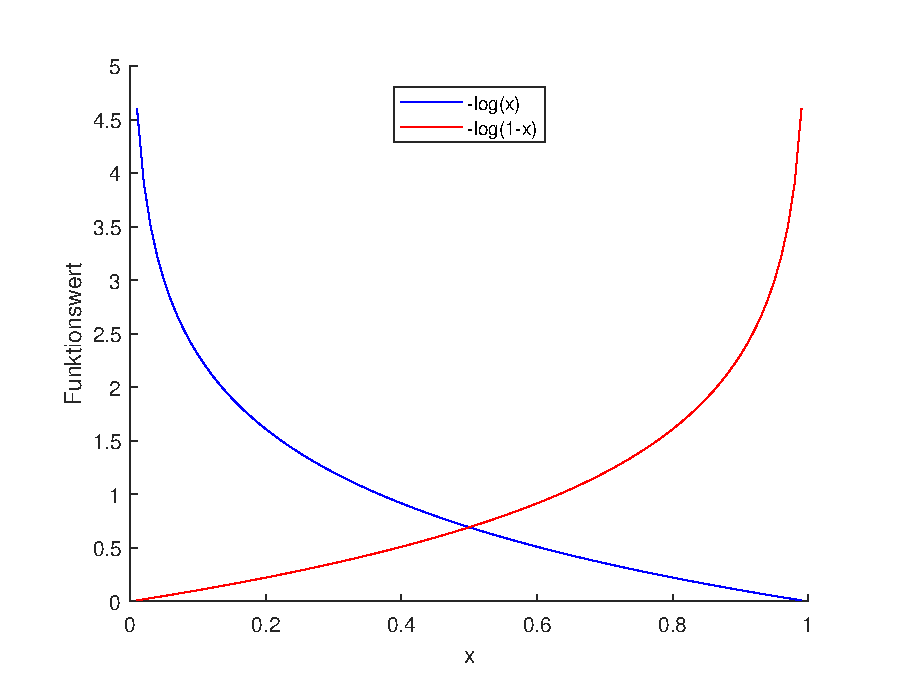
\includegraphics[scale=0.6]{images/plot_costs_logreg.eps}
\caption{Darstellung der Kostenterme der Kostenfunktion für logistische Regression}
\end{figure}
\end{frame}
%\begin{frame}
%\frametitle{Bestimmung der prognostizierten Klasse}
%Sind die Punkte in der Nachbarschaft bestimmt, ergibt sich die prognostizierte Klasse als die Klasse, die am häufigsten in der Nachbarschaft des Punktes vorkommt, formal heißt das
%\[
%\text{predict}(N_k(x)) = \argmax_{y} \sum_{(x_i,y_i)\in N_k(x)} \delta_{(y,y_i)}
%\]
%wobei $\delta_{(y,y_i)} = \begin{cases} 1&, \text{ falls } y = y_i \\ 0 &, \text{ sonst} \end{cases}$ gilt.\\
%Um näher gelegene Punkte stärker einfließen zu lassen, kann die Entscheidung gewichtet werden:
%\[
%\text{predict}(N_k(x)) = \argmax_{y} \sum_{(x_i,y_i)\in N_k(x)} w(x,x_i) \delta_{(y,y_i)}
%\]
%Eine übliche Wahl für die Gewichtung ist etwa $w(x,x_i) = \frac{1}{\Vert x-x_i\Vert}$.
%\end{frame}
\begin{frame}
\frametitle{Kenngrößen zur Bewertung eines Klassifikationsalgorithmus}
Gegeben seien Prognosen für Klassenzugehörigkeiten aus der Testmenge. Wie wird Qualität der Prognosen bestimmt?
\begin{itemize}[<+->]
\item Die möglichen Klassen seien $1$ und $0$
\pause
\item Für jede Prognose in der Testmenge ist der wahre Wert bekannt
\pause
\item Der wahre Wert wird mit $y$ bezeichnet, der prognostizierte Wert mit $\hat{y}$
\pause
\item Dafür werden vier Fälle unterschieden:\\[0.3cm]
\begin{tabular}{c|c|c|c|}
\multicolumn{2}{c}{}&  \multicolumn{2}{c}{Wahre Klasse} \\
 \cline{2-4}
& & $y=1$ & $y=0$ \\
 \cline{2-4}
\multirow{ 2}{*}{Prognose}&$\hat{y}=1$ & true positive & false positive \\  
 & & & (Fehler 1. Art)\\
  \cline{2-4}
&$\hat{y}=0$ & false negative & true negative \\  
 & & (Fehler 2. Art) & \\
  \cline{2-4}
\end{tabular}
\end{itemize}
\end{frame}
\begin{frame}
\begin{itemize}[<+->]
\item Die Angabe \textit{positive} und \textit{negative} bezieht sich auf die Prognose ob die Klasse $1$ (positive) oder $0$ (negative) ist
\item Die Angabe \textit{true} gibt an, dass die Prognose richtig war, entsprechend gibt \textit{false} an, dass die Prognose falsch war
\item \textit{true positive} (kurz tp) heißt, dass das Objekt zur Klasse $1$ zugeordnet wurde und dass diese Zuordnung stimmt
\item \textit{true negative} (kurz tn) heißt, dass das Objekt zur Klasse $0$ zugeordnet wurde und dass diese Zuordnung stimmt
\item \textit{false positive} (kurz fp) heißt, dass das Objekt zur Klasse $1$ zugeordnet wurde und dass diese Zuordnung falsch ist
\item \textit{false negative} (kurz fn) heißt, dass das Objekt zur Klasse $0$ zugeordnet wurde und dass diese Zuordnung falsch ist
\end{itemize}
\end{frame}
\begin{frame}
\frametitle{Precision, Recall und F1-Score}
Nach der Auswertung der Testmenge stehen folgende Werte zu Verfügung:
\begin{tabular}{|c|c|c|c|}
\hline 
 & $ y = 1 $ & $y = 0$ & $\sum$ \\ 
\hline 
$\hat{y} = 1 $& tp & fp & tp+fp \\ 
\hline 
$\hat{y} = 0 $ & fn & tn & fn+tn \\ 
\hline 
$\sum$ & tp+fn & fp+tn & tp+fp+fn+tn \\ 
\hline 
\end{tabular}\\
Daraus lassen sich die folgenden Kennwerte berechnen:
\begin{align*}
\text{precision} &= \frac{tp}{tp+fp}\\
\text{recall} &= \frac{tp}{tp+fn}\\
\text{F1} &= 2 \cdot\frac{\text{precision}\cdot\text{recall}}{\text{precision}+\text{recall}}
\end{align*} 
\end{frame}
\begin{frame}
precision: 
\begin{itemize}[<+->]
\item Anteil der korrekt positiv klassifizierten Instanzen an den insgesamt positiv klassifizierten Instanzen
\item Ein Wert von 1 bedeutet, dass alle positiv klassifizierten Instanzen auch wirklich zur Klasse $1$ gehören
\item Ein Wert von 0 bedeutet, dass keine Instanz, die als positiv klassifiziert wurde, auch wirklich zur Klasse $1$ gehört
\end{itemize}
recall:
\begin{itemize}[<+->]
\item Anteil der korrekt positiv klassifizierten Instanzen an den wirklich positiven Instanzen
\item Ein Wert von 1 heißt, dass alle Instanzen der Klasse $1$ auch als solche erkannt wurden
\item Ein Wert von 0 heißt, dass keine Instanz der Klasse $1$ als solche erkannt wurde
\end{itemize}
F1-Score:
\begin{itemize}[<+->]
\item Harmonisches Mittel von precision und recall
\item Nimmt Werte zwischen 1 (perfekter precision und perfekter recall) und 0 (einer der beiden Werte ist 0) an
\end{itemize}
\end{frame}
\begin{frame}
\begin{itemize}[<+->]
\item precision, recall und F1-Score berücksichtigen nicht die true negative Werte
\item Die bekannte \textit{accuracy} berücksichtigt diese Werte:
\[ \text{accuracy} = \frac{tp+tn}{tp+fp+fn+tn} \]
\item Aber jede der vier Größen ist anfällig für schiefe Verteilungen
\item Ein Maß, das die Größen berücksichtigt, ist der Korrelationskoeffzient von Matthew (engl. Matthews correlation coefficient):
\[
MCC = \frac{tp\cdot tn - fp\cdot fn}{\sqrt{(tp+fn)(fp+tn)(tp+fp)(fn+tn)}}
\]
\item Der Wertebereich vom MCC ist $[-1,1]$, wobei 1 der beste und -1 der schlechteste Wert ist
\item Ein Wert von 0 bedeutet, dass der Klassifikator nicht besser ist, als eine zufällige Prognose
\item Neben den hier vorgestellten Kennwerten existiert noch eine Vielzahl anderer Kennwerte, die eingesetzt werden können
\end{itemize}
\end{frame}
\begin{frame}
Um ein Gefühl für die fünf Kennzahlen zu erhalten, betrachten wir ein hypothetisches Beispiel:
\begin{itemize}[<+->]
\item Es seien $200$ Bauteile untersucht worden, von denen $170$ funktionsfähig und $30$ defekt waren
\item Es sei \[y = \begin{cases} 1 &,\text{falls Bauteil funktionsfähig} \\ 0 &,\text{falls Bauteil defekt}\end{cases}\]
\item Der erste Klassifikator prognostiziert immer Klasse $1$, dann gilt\\
\begin{center}\begin{tabular}{|c|c|c|c|}
\hline 
 & $ y = 1 $ & $y = 0$ & $\sum$ \\ 
\hline 
$\hat{y} = 1 $& 170 & 30 & 200 \\ 
\hline 
$\hat{y} = 0 $ & 0 & 0 & 0 \\ 
\hline 
$\sum$ & 170 & 30 & 200 \\ 
\hline 
\end{tabular}\end{center}
\end{itemize}
\end{frame}
\begin{frame}
Die Kennwerte sind dann
\begin{align*}
\text{precision} &= \frac{170}{200} = 0.85 \\ \text{accuracy} &= \frac{170}{200} = 0.85 \\
\text{recall} &= \frac{170}{170} = 1 \\ \text{F1} &= 2\cdot \frac{0.85\cdot 1}{0.85+1} \approx 0.92
\end{align*}
\pause
ABER: Dieser Klassifikator ist nicht besonders hilfreich, da er die entscheidende Information (Bauteil defekt) nicht liefert!\\
Insbesondere dass der MCC Wert nicht definiert ist, ist ein deutlicher Hinweis darauf, dass der Klassifikator problematisch ist!
\end{frame}
\begin{frame}
Betrachten wir nun einen zweiten Klassifikator, der auch einige Bauteile zur Klasse $0$ zuordnet:
\begin{center}\begin{tabular}{|c|c|c|c|}
\hline 
 & $ y = 1 $ & $y = 0$ & $\sum$ \\ 
\hline 
$\hat{y} = 1 $& 160 & 20 & 180 \\ 
\hline 
$\hat{y} = 0 $ & 10 & 10 & 20 \\ 
\hline 
$\sum$ & 170 & 30 & 200 \\ 
\hline 
\end{tabular}\end{center}
Es gilt:\pause
\begin{align*}
\text{precision} &= \frac{160}{180} \approx 0.89 \\ 
\text{accuracy} &= \frac{170}{200} \approx 0.94 \\
\text{recall} &= \frac{160}{170} \approx 0.94 \\ 
\text{F1} &= 2\cdot \frac{0.89\cdot 0.94}{0.89+0.94} \approx 0.91\\
MCC &= \frac{160\cdot 10 - 10\cdot 20}{\sqrt{170\cdot 30\cdot 180\cdot 20}} \approx 0.33
\end{align*}
\end{frame}
\begin{frame}
\frametitle{$k$ means}
Als letzter Algorithmus soll hier der $k$ means Algorithmus vorgestellt werden.
\begin{itemize}[<+->]
\item $k$ means erstellt $k$ Cluster
\item Dafür wird ein Abstandmaß benutzt
\item Das Vorgehen des $k$ means Algorithmus:
\begin{enumerate}[<+->]
\item Parameter: Wähle $k$ und das Abstandmaß
\item Wähle zufällig $k$ Zentrumspunkte $c_1,\ldots,c_k$, die den gleichen Wertebereich und die gleiche Dimension wie die Datenpunkte besitzen
\item Bestimme für alle Datenpunkte $x_i$ ihren Abstand zu den Punkten $c_1,\ldots,c_k$
\item Der Punkt $x_i$ wird dem Zentrumspunkt $c_j$ zugeordnet (und damit vorläufig dem Cluster $j$), der ihm am nächsten ist
\item $c_j$ wird als der Mittelwert aller Punkte $x_i$ aus dem Cluster $j$ gesetzt
\item Wiederhole Schritte 3-5 solange, bis eine maximale Iterationszahl erreicht wurde, oder die $c_j$ sich nicht mehr ändern
\item Ausgabe: Zuordnung der $x_i$ zu den Clustern $1$ bis $k$
\end{enumerate}
\end{itemize}
\end{frame}
\begin{frame}
\begin{itemize}[<+->]
\item Der Parameter $k$ kann mit der Ellbogen Methode gewählt werden, als Kostenmaß kann hier die Summe aller Abstände der $x_i$ zu ihrem $c_j$ gewählt werden
\item Durch die zufällige Initialisierung der $c_j$ ist die Ausgabe im Allgemeinen \textbf{nicht eindeutig}, daher sollte $k$ means mehrmals wiederholt werden. Am Ende wird die Cluster Zuweisung gewählt, die die kleinsten Kosten aufweist
\item Wie bei allen unüberwachten Algorithmen gibt es hier keine Trainings- oder Testmenge
\end{itemize}
\end{frame}